%Matteo Kumar - Leonard Schatt
% Fortgeschrittenes Physikalisches Praktikum
% Main-Datei für die Auswertung in TeX

% Struktur:
% Für jeden Abschnitt gibt es einen Ordner, damit jeder individuell an seinen Aufgaben arbeiten
% kann, ohne beim merge in GitHub Konflikte zu erhalten. Deshalb werden alle Unteraufgaben auch 
% extra in Ordner angelegt. Die einzelnen Dateien über den input Befehl einfügbar.
% Bilder und andere Grafik werden im Ordner Grafik abgelegt 


% Packages
\documentclass[paper=a4,bibliography=totoc,BCOR=10mm,twoside,numbers=noenddot,fontsize=11pt]{scrreprt}
\usepackage[ngerman]{babel}
\usepackage[latin1, utf8]{inputenc}
\usepackage[babel,german=quotes]{csquotes} %For Quotes
\usepackage[T1]{fontenc}
\usepackage{lmodern}
\usepackage{graphicx}
\usepackage{nicefrac}
\usepackage{fancyvrb}
\usepackage{amsmath,amssymb,amstext}
\usepackage{siunitx}
\usepackage{url}
\usepackage{natbib}
\usepackage{microtype}
\usepackage[format=plain]{caption}
\usepackage{physics}
\usepackage{titleref}

% Zusätzliche Packages
\usepackage{geometry}
\usepackage{anyfontsize}
\usepackage[table]{xcolor}
\usepackage{ifthen}
\usepackage[absolute,overlay]{textpos}
\usepackage{amsfonts}
\usepackage{xstring}
\usepackage{tikz}
\usepackage{pdfpages}
\usepackage{booktabs}
\usepackage{hyperref}

% Abschnittseinrückung und -abstand
% Die folgenden Zeilen sollen möglichst nicht verändert werden
\parindent 0.0cm
\parskip 0.8ex plus 0.5ex minus 0.5ex

% Anzahl und Größe von Gleitobjekten
% maximal 2 Objekte oben und unten
% erlaubt auch größere Bilder, welche die ganze Seite benötigen
% Die folgenden Zeilen sollen möglichst nicht verändert werden
\setcounter{bottomnumber}{2}
\setcounter{topnumber}{2}
\renewcommand{\bottomfraction}{1.}
\renewcommand{\topfraction}{1.}
\renewcommand{\textfraction}{0.}

%\sc und \bc veraltet. Daher: (20.09.2018)
\DeclareOldFontCommand{\sc}{\normalfont\scshape}{\@nomath\sc}
\DeclareOldFontCommand{\bf}{\normalfont\scshape}{\textbf}

% Verschiedenes
\pagestyle{headings}          % Der Seitenstil sollte möglichst nicht verändert werden
\graphicspath{{./bilder/}}    % Der Pfad für die Abbildungen Abbildungen wird gesetzt
\VerbatimFootnotes            % \verb etc.

% Funktionen
\newcommand\tab[1][1cm]{\hspace*{#1}}
\newcommand{\vect}[1]{\boldsymbol{\mathbf{#1}}}
\newcolumntype{g}{>{\columncolor[rgb]{ .741,  .843,  .933}}l}
% Tiefgestellte Zahlen nicht kursiv
\catcode`_=\active
\newcommand_[1]{\ensuremath{\sb{\mathrm{#1}}}}

\begin{document}

    \nonfrenchspacing

    % 0. Kapitel 
    %Matteo Kumar - Leonard Schatt
% Fortgeschrittenes Physikalisches Praktikum
% 0. Cover
% Noch abänderbar nur ein Vorschlag
\newgeometry{top=30mm, bottom=20mm, inner=20mm, outer=20mm}
\thispagestyle{empty}

% Colors
\definecolor{Notablue}{HTML}{3498DB}		%Theoretische Physik
\definecolor{Notared}{HTML}{CF366C}			%Mathematik
\definecolor{Notagreen}{HTML}{19B092}		%Experimentalphysik
\definecolor{Notaorange}{HTML}{FA9D00}		%Chemie/Wahlfach nicht physikalisch
\definecolor{Notagrey}{HTML}{969696}		%Praktikum
\definecolor{Notalavendel}{HTML}{9DBBD8}	%Wahlfächer physikalisch

% Boolean by default false
\newboolean{twoRows}
\newboolean{symbol}

% Funktions
\makeatletter
   \def\vhrulefill#1{\leavevmode\leaders\hrule\@height#1\hfill \kern\z@}
\makeatother
\newcommand*\ruleline[1]{\par\noindent\raisebox{.8ex}{\makebox[\linewidth]{\vhrulefill{\linethickness}\hspace{1ex}\raisebox{-.8ex}{#1}\hspace{1ex}\vhrulefill{\linethickness}}}}

% Variables
\def\schriftgrosse{70}
\def\linethickness{1,5pt}

\def\farbe{Notagrey}
\def\fach{PPB2}
\def\name{Matteo Kumar - Leonhard Schatt}
\def\uberschrift{FRET} % Absatz mit \\[0,5cm]; u = Übung, k = Klausur; s = Skript, e = Ergebnis
\def\bottom{WS2021}
\def\datum{27.09.2021}
\def\platz{NW I    }
\def\betreuer{Chenyu Jin}
\def\groupnr{3}

\begin{titlepage}
			
	\centering
	{\LARGE \sffamily {\textbf{\bottom}\par}}
	\vspace{2,5cm}
    {\fontsize{40}{0}\sffamily\ruleline{\textcolor{\farbe}{\textbf{\fach}}}\par}
    \vspace{6cm}
	{\Large\sffamily \ruleline{\name}\par}
	
	
	% Choose Text
	\ifthenelse{\equal{\uberschrift}{s}} {\def\titel{Skript}}	
		{\ifthenelse{\equal{\uberschrift}{k}} {\def\titel{Klausur}}
			{\ifthenelse{\equal{\uberschrift}{u}} {\def\titel{Übung}}
				{\ifthenelse{\equal{\uberschrift}{e}} {\def\titel{Klausur \\[0,5cm] Ergebnis}}
					{\def\titel{\uberschrift}}
				}
			}
		}
	
	\begin{textblock*}{21cm}(0cm,9cm) % {block width} (coords), centered		
		{\fontsize{\schriftgrosse}{0}\sffamily\textcolor{\farbe}{\textbf{\titel}}\par}
	\end{textblock*}
	
	% Choose Logo
	\ifthenelse {\equal{\farbe}{Notared}} {\def\logo{Bilder/Logo/UniBTNotared}}
		{\ifthenelse {\equal{\farbe}{Notagreen}} {\def\logo{Bilder/Logo/UniBTNotagreen}}
			{\ifthenelse {\equal{\farbe}{Notablue}} {\def\logo{Bilder/Logo/UniBTNotablue}}
				{\ifthenelse {\equal{\farbe}{Notaorange}} {\def\logo{Bilder/Logo/UniBTNotaorange}}
					{\ifthenelse {\equal{\farbe}{Notagrey}} {\def\logo{Bilder/Logo/UniBTNotagrey}}
						{\ifthenelse {\equal{\farbe}{Notalavendel}} {\def\logo{Bilder/Logo/UniBTNotalavendel}}	
							{\ifthenelse {\equal{\farbe}{black}} {\def\logo{Bilder/Logo/UniBT}}	
								{\def\logo{noLogo}}
							}
						}
					}
				}
			}
		}	

	\IfSubStr{\logo}{noLogo}{\setboolean{symbol}{false}}{\setboolean{symbol}{true}}
	
	% Gruppe
	\vspace{10cm}
	{\large\sffamily{Gruppe \groupnr}}
	
	%Logo
	\vfill

	\ifthenelse{\boolean{symbol}}
		{
			\begin{figure}[h]
			\begin{center}
				
				\includegraphics[width=2cm]{\logo}
				
			\end{center}
			\end{figure}
		}
	
\end{titlepage}

\restoregeometry

% Information
\chapter*{Informationen}
\label{chap:info}

\begin{tabular}{l l}

	{\textbf{Versuchstag}} \hspace{1cm} & \hspace{1cm} {\datum}\\[0,2cm]
	{\textbf{Versuchsplatz}} \hspace{1cm} & \hspace{1cm} {\platz}\\[0,2cm]
	{\textbf{Betreuer}} \hspace{1cm} & \hspace{1cm} {\betreuer}\\[1,2cm]
	{\textbf{Gruppen Nr.}} \hspace{1cm} & \hspace{1cm} {\groupnr}\\[0.2cm]
%	{\textbf{Auswertperson}} \hspace{1cm} & \hspace{1cm} {\auswertp}\\[0.2cm]
%	{\textbf{Messperson}} \hspace{1cm} & \hspace{1cm} {\messp}\\[0.2cm]
%	{\textbf{Protokollperson}} \hspace{1cm} & \hspace{1cm} {\protop}\\[0.2cm]

\end{tabular}

    \thispagestyle{empty}
    \cleardoublepage
    \tableofcontents
    \cleardoublepage

    % 1. Kapitel Einleitung
    %Matteo Kumar - Leonard Schatt
% Fortgeschrittenes Physikalisches Praktikum

% 1. Kapitel Einleitung

\chapter{Einleitung}
\label{chap:einleitung}

Der Laser ist eines der wichtigsten Geräte, wenn es um optische Untersuchungen in Laboren geht. Nicht nur sein Gaußprofil 
und seine konstante Leistung, sondern auch sein schmalbandiger Frequnzbereich machen ihn zu einem in den Naturwissenschaften
Untersuchungsmittel. Dabei ist das Wissen zu Lasern in der breiten Bevölkerung eher durch Popkultur wie die Starwar-Reihe geprägt.
Das viele der dortigen Anwendungen von Laserlicht unsinnig sind, sollte nach dem Versuch jedem klar sein, denn jeder, der einen Laser mal
justiert hat, weiß, dass dieser einem sicher ausgehen würde, wenn man diesen in ein Schwert bauen würde und dieses massiven Erschütterungen aussetzten
würde. Das Hologram hingegen ist, wie wir in diesem Versuch sehen werden, kein reines Fantasieprodukt von Autoren.
Dieses werden wir am Ende des Versuches an einem echten Hologram bestätigt bekommen.

    % 2.Kapitel Fragen zur Vorbereitung
    %Matteo Kumar - Leonard Schatt
% Fortgeschrittenes Physikalisches Praktikum
 

% Matteo Kumar
% PPB2 Solarzelle
%Grundlagen

\chapter{Grundlagen}
\section{Bändermodell und Halbleiter}
\subsection{Leitfähigkeit im Bändermodell}
Will man die Leitfähigkeit von Materialien anschaulich betrachten, ist das sog. Bändermodell hilfreich, das die erlaubten Energiezustände in einem Festkörper beschreibt. Jedes Band kann eine endliche Zahl an Ladungträgern enthalten; ist das Band voll besetzt, trägt es nicht zur Leitfähigkeit bei, da keine freien Energieniveaus existieren, um Energie aus einem elektrischen Feld aufzunhemen. Für die Leitfähigkeit wichtig sind vor allem das Valenzband und das Leitungsband. Das Leitungsband ist das energetisch niedrigste Band, das bei tiefen Temperaturen nicht voll besetzt ist; das Valenzband ist das unmittelbar darunter liegende Band. (\cite{Eichler2001}, S. 299f)
Elektrische Leiter haben bereits bei sehr niedrigen Temperaturen Ladungsträger im Leitungsband, weshalb sie im Allgemeinen immer leitend sind. Halbleiter und Isolatoren hingegen haben diese Eigenschaft nicht. Der Unterschied zwischen diesen beiden liegt in der Breite sog. Bandlücke, der energetische Abstand zwischen Valenz- und Leitungsband. Während die Bandlücke von Isolatoren sehr breit ist, ist die von Halbleitern hinreichend schmal, sodass bei geringen (z.B. thermischen) Energien Ladungsträger aus dem Valenz- in das Leitungsband wechseln können und so den Halbleiter leitend machen. \\
\begin{figure}[h]
    \centering
    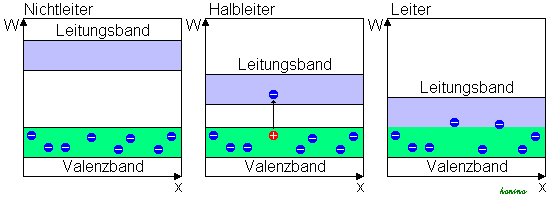
\includegraphics[scale=0.75]{Bilder/Baendermodell.png}
    \caption{Bändermodell für Nichtleiter, Halbleiter und Leiter \protect \footnotemark}
\end{figure}

\footnotetext{\url{https://www.virtualuniversity.ch/elektronik/analog/halbleiter/1.html}, Stand: 9.9.21}


\subsection{Dotierung von Halbleitern und pn-Übergang}
Die Leitfähigkeit von Halbleitern lässt sich durch Dotierungen verbessern. Man hat hierzu zwei Möglichkeiten: p- und n-Dotierung. \\
Bei der n-Dotierung werden Atome mit einem Valenzelektron mehr als die des Halbleitermaterials eingebracht. Dies hat zur Folge, dass das 
überschüssige Elektron bereits mit thermischen Energien in das Leitungsband angeregt werden kann. Die Leitfähigkeit wird erhöht und es 
bleibt ein positiv geladener Atomrumpf zurück.\\
Die p-Dotierung bedient sich des umgekehrten Prinzips. Das Halbleitermaterial wird mit einer Atomsorte mit einem Elektron weniger 
verunreinigt. Das Fehlelektron wird auch als "Loch" bezeichnet. Dieses Loch hat eine hohe Elektronenaffinität, weshalb es ein Elektron 
von einem Atom des Halbleiters bindet, das nun wiederum ein Loch hat. Diese Leitungsart wird auch als Lochleitung bezeichnet. 
Im Gegensatz zur n-Dotierung bleibt hier ein negativ geladener Atomrumpf zurück. 
(\cite{Goebel2019} S. 7-11). Bei einer Dotierung verschiebt sich auch die Fermienergie, 
die im Falle eines undotierten Leiters ungefähr in der Mitte zwischen Unterkante des Leitungsbandes und Oberkante des Valenzbandes 
liegt. Im Falle einer n-Dotierung verschiebt sich die Fermienergie aufgrund der zusätzlichen Elektronen im Valenzband nach oben, 
im Falle einer p-Dotierung aufgrund der zusätzlichen Löcher nach unten. (\cite{Wellmann2019}, S.60)\\
Fügt man nun einen p- und einen n-dotierten Halbleiter zusammen, erhält man einen sogenannten pn-Übergang. Im p-dotierten Halbleiter 
herrscht ein Löcherüberschuss und im n-dotierten ein Elektronenüberschuss. Aufgrund dieses Konzentrationsgefälles wandern Elektronen 
und Löcher und rekombinieren, bis sich ein Gleichgewicht einstellt. Nun existiert direkt am Übergang zwischen den Materialien eine 
Zone, in der es keine freien Ladungsträger mehr gibt. Es liegen nur noch die negativ bzw. positiv geladenen Atomrümpfe vor, die 
ihrerseits wieder eine Potentialdifferenz verursachen.\\
Legt man nun ein externes Feld an, kann, je nach Anlegrichtung, diese Differenz entweder vergrößert werden und es fließt kein Strom, 
die Sperrzone vergrößert sich, oder sie wird verringert bis sie schließlich überwunden wird. Es existiert ein Stromfluss. \\
Dies kann auch im Bändermodell betrachtet werden: Durch die Rekombination von freien Löchern und Elektronen in der Verarmungszone 
gleichen sich die Fermienergien beider Materialien an. Dabei verbiegt sich das Band und es entsteht eine Potentialdifferenz zwischen 
p- und n-dotiertem Halbleiter. \\

\begin{figure}[h]
    \centering
    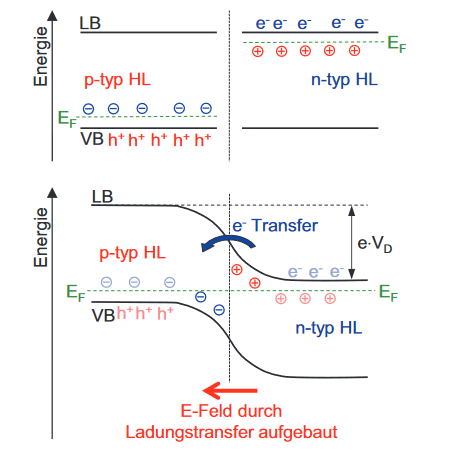
\includegraphics[scale=0.75]{Bilder/Bandverbiegung.png}
    \caption{Bei einem pn-Übergang gleichen sich die Fermienergien (in grün) an. Dadurch verbiegt sich das Band und es entsteht eine 
    Potentialdifferenz \protect \footnotemark}
\end{figure}

\footnotetext{\cite{Wellmann2019}, S.62}

\begin{figure}[h]
    \centering
    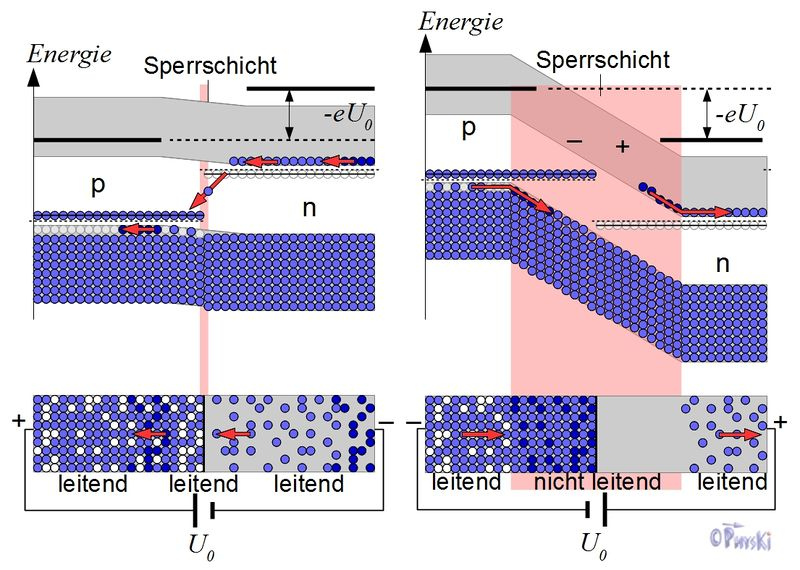
\includegraphics[scale=0.5]{Bilder/DurchlassSperr.jpg}
    \caption{pn-Übergang mit angelegter Spannung in Durchlass- (links) bzw. Sperrrichtung (rechts) \protect \footnotemark}
\end{figure}

\footnotetext{\url{https://www2.physki.de/PhysKi/index.php/Pn-%C3%9Cbergang}, Stand: 19.09.21}


\clearpage


\section{Solarzelle}
\subsection{Funktionsweise}
Der Typ von Solarzelle, mit dem sich in diesem Versuch beschäftigt wird, besteht im Wesentlichen aus einem pn-Übergang. 
Trifft nun Licht, also Photonen, auf die Zelle, werden dadurch freie Elektronen-Löcher-Paare erzeugt. Im einfachsten Fall werden diese 
durch den Drift des elektrischen Feldes der Atomrümpfe in der Verarmungszone separiert und wandern in Richtung der aufgebrachten 
Kontakte; ein Strom kann abgegriffen werden. Manche Zellen nutzen zusätzlich noch die durch die Konzentrationsgefälle der Elektronen 
und Löcher bedingte Diffusion. (\cite{Shah2020}, S.46) Unbeleuchtete Solarzellen unterscheiden sich also im 
prinzipiellen Aufbau nicht von einfachen Dioden; entsprechend stimmt auch der Verlauf ihrer U/I-Kennlinien überein. Wird die Zelle nun 
beleuchtet, bedingen die entstehenden Elektron-Löcher-Paare einen Kurzschlussstrom; die Kennlinie verschiebt sich im Vergleich zur 
Diode in negative I-Richtung. \\

\begin{figure}[h]
    \centering
    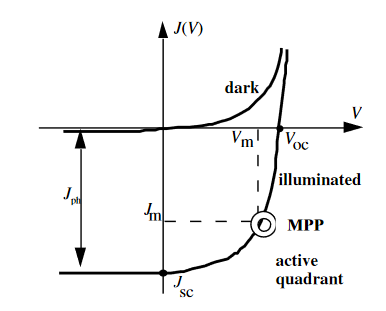
\includegraphics[scale=0.75]{Bilder/Kennlinien.png}
    \caption{U/I-Kennlinie einer Solarzelle für den beleuchteten und unbeleuchteten Fall \protect \footnotemark}
    \label{bild:kennlinien}
\end{figure}

\footnotetext{\cite{Shah2020}, S.50}


\subsection{Ersatzschaltbild}
Die ideale Solarzelle kann durch eine Stromquelle, die den Photostrom modelliert, und eine Diode dargestellt werden. 
Erweitert werden kann dieses Modell durch einen Serienwiderstand, der hauptsächlich Widerstände in den Kontakten und Verkabelungen
widerspiegelt, und einen Parallelwiderstand, der alle Effekte im Kristall zusammenfasst, die den pn-Übergang überbrücken.
(\cite{Shah2020}, S.52f)
Das Ersatzschaltbild in Abb. \ref{bild:ersatzschaltbild} zu finden.

\begin{figure}[h]
    \centering
    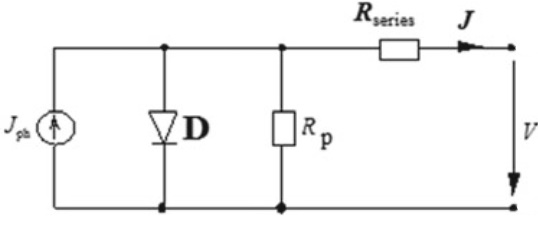
\includegraphics[scale=0.5]{Bilder/Ersatzschaltbild.png}
    \caption{Ersatzschaltbild einer Solarzelle \protect \footnotemark}
    \label{bild:ersatzschaltbild}
\end{figure}
\footnotetext{\cite{Shah2020}, S.53}

Die sich daraus ergebende U/I-Kennlinie wird durch die Shockley-Gleichung beschrieben:
\begin{equation}
    I = I_0 (exp(\frac{q(U-R_SI)}{nkT})-1) + \frac{U-R_SI}{R_P} - I_{Ph}
\end{equation}

(\cite{Gerken2021}, S.3)

\subsection{Wichtige Kenngrößen}
Die Leistung berechnet sich nach $P = |UI|$, im U/I-Diagramm entspricht ihr also die Fläche des Rechtecks unter der Kennlinie. Am Maximum-Power-Point $MPP$ ist $P$ maximal. Der $MPP$ ist auch in Abb. \ref{bild:kennlinien} eingezeichnet. \\
Der Wirkungsgrad einer Solarzelle berechnet sich aus dem Verhältnis der nutzbaren und der einfallenden Leistung:
\begin{equation*}
\eta = \frac{P_{MPP}}{P_{ein}} = \frac{|UI|_{MPP}}{P_{ein}}
\end{equation*}
Ein weiterer Gütefaktor einer Solarzelle ist der Füllfaktor $FF$. Er ist das Verhältnis der Leistung am $MPP$ und des Produktes aus Leerlaufspannung $U_{OC}$ und Kurzschlussstrom $I_{SC}$. Eine ideale Solarzelle hat den Füllfaktor $1$, eine reale $FF < 1$.

\begin{equation*}
FF = \frac{|UI|_{MPP}}{U_{OC} I_{SC}}
\end{equation*}
Die Externe Quanteneffizienz $EQE$ einer Solarzelle beschreibt das Verhältnis von Photonen, die zum Photostrom beitragen, zu einfallenden Photonen. Man kann sie also auch als Wirkungsgrad bezogen auf Photonen betrachten; im Idealfall gilt $EQE = 1$. Es folgt:

\begin{equation}
EQE = \frac{Photonen \, im \, Photostrom}{einfallende \, Photonen} = \frac{ \frac{I_{Ph}t}{e}}{r_{ein}t} = \frac{I_{Ph}}{e \, r_{ein}} = \frac{I_{Ph} h \nu}{e P_\lambda}
\end{equation}

wobei im letzten Schritt angenommen wurde, dass das einfallende Licht monochromatisch ist, und $P_\lambda$ die einfallende Strahlungsleistung ist. \\
Schreibt man nun die Frequenz in die Wellenlänge um, erhält man:

\begin{equation}
EQE = \frac{h c}{e} \frac{I_{Ph}}{\lambda P_\lambda} = \frac{h c}{e} \frac{SE(\lambda)}{\lambda}
\end{equation}

Im letzten Schritt wurde hierbei ausgenutzt, dass der Vorfaktor konstant ist, um die Spektrale Empfindlichkeit $SE(\lambda) = \frac{I_{Ph}}{P_\lambda}$ zu definieren.

\subsection{Im Versuch verwendete Solarzelltypen}
Der Unterschied zwischen den im Versuch vorliegenden Silizium- und Kupfer-Indium-Selenoid-(CIS-)Zellen liegt in der Art der Bandlücke der 
jeweiligen Materialien. CIS-Zellen haben eine sogenannte direkte Bandlücke; auftreffende Photonen können direkt absorbiert werden. 
Dagegen haben Siliziumzellen eine indirekte Bandlücke; Photonen können erst durch eine Interaktion mit einem geeigneten Phonon 
absorbiert werden, weshalb die Absorptionswahrscheinlichkeit im Vergleich zur CIS-Zelle deutlich herabgesetzt ist. Aufgrund dessen sind 
bei Siliziumzellen wesentlich dickere Halbleiterschichten oder spezielle Lichtfallen nötig, um die Stromausbeute zu erhöhen 
(\cite{Shah2020}, S.40). \\
Des Weiteren werden im Versuch zwei verschiedene Arten von Siliziumzellen verwende: Mono- und multikristalline. Monokristalline 
Solarzellen bestehen aus einem einzigen gewachsenem Kristall, im Gegensatz zu polykristallinen Solarzellen. Die Herstellung von 
Einkristallen ist zwar wesentlich aufwändiger und kostenintensiver, jedoch kann das Solarmodul bei Verwendung dieser einen deutlich 
höheren Wirkungsgrad erzielen. (\cite{Altekrueger2008}, S.26ff)
Die Lage der Bandkanten sind für Silizium $1,1242$eV 
(\url{https://www.pveducation.org/pvcdrom/materials/general-properties-of-silicon}, Stand: 9.9.21) und für CIS $1,02$eV 
(\url{https://www.pveducation.org/pvcdrom/materials/cuinse2}, Stand: 9.9.21).
 % Frage 13

 \section(Sonnenspektrum)
 
 In erster Näherung kann das Spektrum der Sonne als das eines schwarzen Strahlers beschrieben werden. Auf dem Weg zur Erde wird allerdings 
 ein Teil der Strahlung beispielsweise in der Atmosphäre reflektiert oder absorbiert, sodass hier nur ein reduziertes Sonnenspektrum 
 gemessen wird. Ein Vergleich der Spektren findet sich in Abb. \ref{bild:Sonnenspektrum}. % QUELLE!!

 \begin{figure}[h]
    \centering
    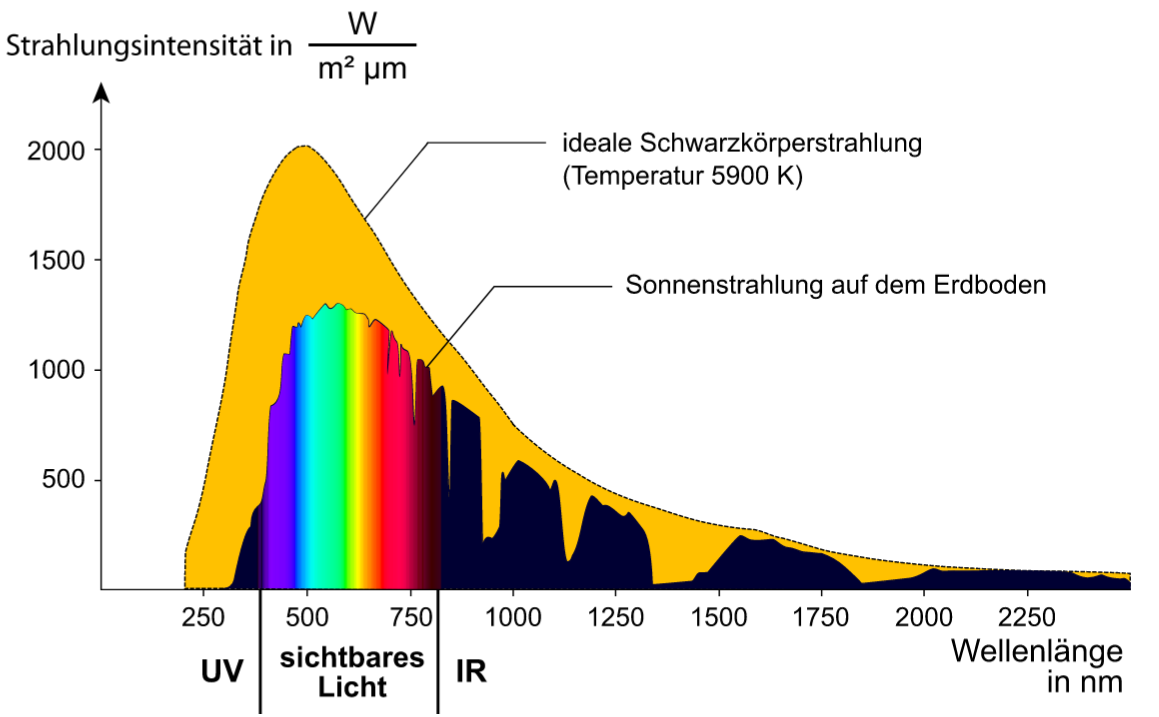
\includegraphics[scale=0.5]{Bilder/Sonnenspektrum.png}
    \caption{Ersatzschaltbild einer Solarzelle \protect \footnotemark}
    \label{bild:Sonnenspektrum}
\end{figure}
\footnotetext{\url{https://www.leifiphysik.de/astronomie/sonne/grundwissen/sonnenspektrum}, Stand: 20.09.21}




    % 3.Kapitel Protokoll
    %% Charlotte Geiger - Manuel Lippert - Leonard Schatt
% Physikalisches Praktikum

% 3.Kapitel  Protokoll

% Variables



% Leonhard Schatt

\chapter{Methodik}



% Einbindung des Protokolls als pdf (mit Seitenzahl etc.)
% Erste Seite mit Überschrift
%\includepdf[pages = 1, landscape = false, nup = 1x1, scale = \skalierung , pagecommand={\thispagestyle{empty}\chapter{Protokoll}}]
%            {03-Protokoll/Protokoll.pdf}
% Restliche Seiten richtig skaliert
%\includepdf[pages = -, landscape = false, nup = 1x1, scale = \skalierung , pagecommand={}]
%            {03-Protokoll/Protokoll.pdf}

    % 4.Kapitel Versuchsauswertung
    % Matteo Kumar - Leonard Schatt
% Fortgeschrittenes Physikalisches Praktikum
% 4.Kapitel Versuchsauswertung

\chapter{Auswertung und Diskussion}
\label{chap:versuchsauswertung}

% Text

% Input der Teilauswertung je nach Produktion der Nebendateien ohne Ordner


\section{Transversalmoden eines Lasers}
\label{section:transvM}

Ein Laser hat mehrere Moden. Normalerweise ist die $TEM_{00}$-Mode dominant, das heißt man sieht einen zusammenhängenden 
Punkt mit näherungsweise gaußförmigem Profil. Es gibt jedoch auch noch andere Moden, wie in dem Grundlagenkapitel \ref{subs:moden}
beschrieben. Diese haben wir versucht zu erzeugen, indem wir ein eine dünne Drahtblende einbringen, nachdem wir den Laser in 
konfokaler Spiegelstellung justiert haben. Dann verschieben wir die Drahtblende so lange, bis wir eine Veränderung des Punktes auf einem circa 
50\,cm entfernten Schirm sehen können. Dabei haben wir die in Abbildung \ref{bild:Moden} gezeigten Moden beobachtet.
\begin{figure}[ht]
    \centering
    \subfloat[$TEM_{00}$]{\label{TEM00}%
      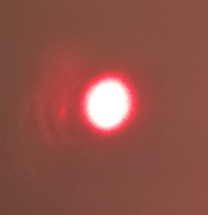
\includegraphics[width=0.235\textwidth]
      {Bilder/Auswertung/TEM00.png}}\quad
    \subfloat[$TEM_{10}$]{\label{TEM10}
      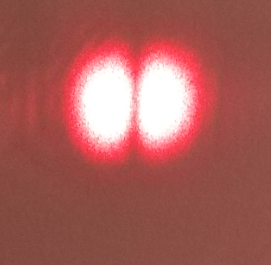
\includegraphics[width=0.25\textwidth]
      {Bilder/Auswertung/TEM10.png}}\quad
    \subfloat[$TEM_{01}$]{\label{TEM01}%
      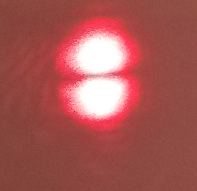
\includegraphics[width=0.25\textwidth]
      {Bilder/Auswertung/TEM01.png}}\quad
    \subfloat[$TEM_{20}$]{\label{TEM20}%
      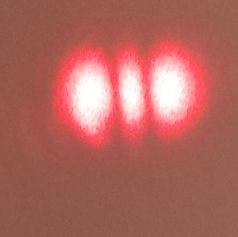
\includegraphics[width=0.25\textwidth]
      {Bilder/Auswertung/TEM20.png}}\quad
      \subfloat[$TEM_{30}$]{\label{TEM30}%
      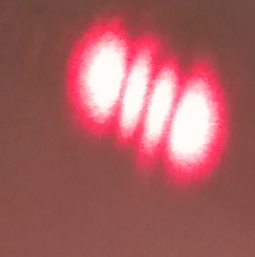
\includegraphics[width=0.25\textwidth]
      {Bilder/Auswertung/TEM30.png}}\quad
      \subfloat[$TEM_{un.}$]{\label{TEMunz}%
      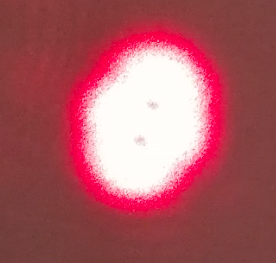
\includegraphics[width=0.25\textwidth]
      {Bilder/Auswertung/TEMunsugeordnet.png}}
      \subfloat[$TEM_{01*}$]{\label{TEM01*}\quad
      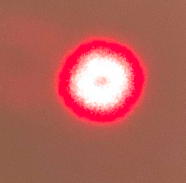
\includegraphics[width=0.245\textwidth]
      {Bilder/Auswertung/TEM11.png}}
      \caption{Transversalmoden der HeNe-Laser}
      \label{bild:Moden}
  \end{figure}

  Dabei konnten wir die klassischen $TEM$-Moden mit polarisierenden Elementen, welche die Symmetrie des Resonators aufhebt, beobachten.
  Spannenderweise kann in Abbildung \ref{TEM01*} auch eine radialsymmetrischen Mode beobachten werden. Außerdem
  gibt es eine Mode in \ref{TEMunz}, welche wir nicht identifizieren konnten. Diese könnte eine Mischmode sein.
\clearpage
\section{Axiale Lasermoden}

In diesem Teil beschäftigen wir uns mit den axialen Lasermoden. Dafür verwenden wir ein durchstimmbares konfokales Fabry-Pérot-Interferometer. 
Dazu führt man den Laser möglichst parallel in das Interferometer. Die vom Fabry-Pérot-Interferometer durchgelassene Intensität wird dann von einer 
Photodiode detektiert, verstärkt um einen Faktor 100 und dann grafisch dargestellt. Die Rampenspannung des Interferometers wird dann so eingestellt, 
das man 2 mal den freien Spektralbereich sieht. Dies erkennt man daran, dass man genau zwei mal das gleiche Bild nebeneinander auf dem Oszilloskop sieht. 
Den Abstand der Lasermoden bestimmen wir einfach durch Ablesen am Oszilloskop. Zuvor müssen wir aber herausfinden, wie das Zeitsignal auf der 
x-Achse des Oszilloskops mit der Frequenz zusammenhängt.\\

Dazu nehmen wir zwei mal den selben Peak, aber in zwei nebeneinanderliegenden Darstellungen auf Channel 1 in Abbildung \ref{bild:FreierSpektralbereich}.
Dieser Abstand entspricht dem freien Spektralbereich des Interferometers. Dieser ist bei dem hier verwendeten Gerät 2\,GHz. Man könnte ebenfalls das Triggersignal verwenden, 
aber an den Peaks kann man das Maximum leichter ablesen. Man erhält also den Umrechnungsfaktor 

\begin{equation*}
    m = (152 \pm 7)\,\frac{\mathrm{MHz}}{\mathrm{ms}}
\end{equation*}

für die Umrechnung 

\begin{equation}
    \Delta \nu = m\cdot \Delta t
    \label{eq:Umrechnung}
\end{equation}

von der vom Oszilloskop ausgegebenen Zeitdifferenz in Frequenzen $\nu$.


\begin{figure}[ht]
    \centering
    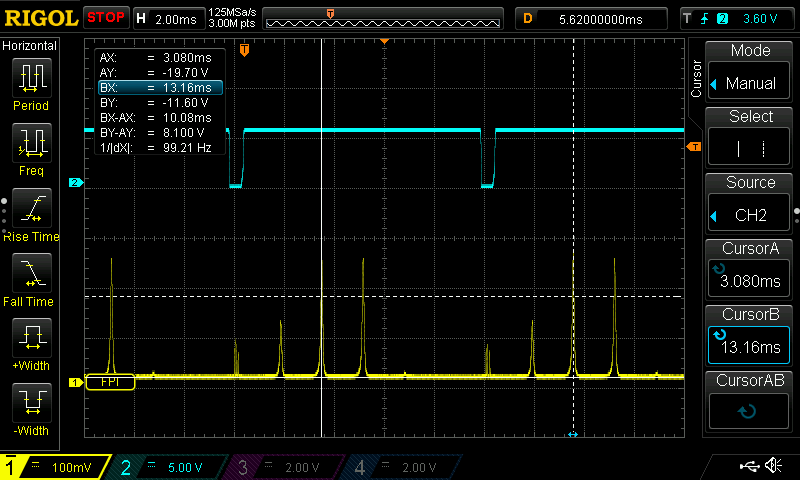
\includegraphics[width = \linewidth]{Bilder/Auswertung/FabryPerotKalibr.png}
    \caption{Longitudinale Lasermoden mit dem Fabry-Pérot aufgenommen. Channel 1 ist das Messsignal und Channel 2 ist des Triggersignal des Interfermoters. Gekennzeichnet sind 
    mit den x-Marker zwei gleich Peaks.}
    \label{bild:FreierSpektralbereich}
\end{figure}


\subsection*{Abstand und Linienbreite Axialer Lasermoden}

Den Abstand der Moden bestimmt man auch grafisch aus Abbildung \ref{bild:AxialModenAbstand}. Aus diesem erhält man 
\begin{equation*}
    \Delta t = (1,660 \pm 0,086)\,\mathrm{ms}
\end{equation*}
und mit der Umrechnung aus Gleichung \ref{eq:Umrechnung} erhalt man 

\begin{equation}
    \textcolor{red}{\delta \nu = (252 \pm 17)\,\mathrm{MHz}}
    \label{eq:Modenabstand}
\end{equation}

den Abstand zweier longitudinaler Lasermoden. Die Unsicherheit wird hierbei aus geschätzter Ableseunsicherheit und
der Unsicherheit der Kalibrierung  mittels Fehlerfortpflanzung berechnet. Auf selbe Weise wird 

\begin{equation}
    \textcolor{red}{\Delta \nu_{multi} = (13,3 \pm 1,5)\,\mathrm{MHz}}
\end{equation}

auch die Linienbreite (FWHM) aus Abbildung \ref{bild:Lininebreite} bestimmt. Gleiches tun wir auch für die einzelne Mode
aus Abbildung \ref{bild:LininebreiteSingle}. Damit erhalten wir die Werte, welche in Tabelle \ref{tab:Linienbreite} dargestellt sind.

\begin{table}
    \centering
 
    \begin{tabular}{lcr}
        \toprule
        Messgröße & Symbol & Wert in MHz\\
        \midrule
        Freier spektraler Bereich& $\Delta \nu_{FSB}$ & 2000\\
        Modenabstand& $\delta\nu$& $252 \pm 17$\\
        FWHM (multi-mode)& $\Delta\nu_{multi}$&$13,3 \pm 1,5$\\
        FWHM (single)& $\Delta\nu_{multi}$&$16,7 \pm 2,6$\\
        \bottomrule        
    \end{tabular}
  
    \caption{Freier spektraler Bereich, Modenabstand, Halbwertsbreite des He-Ne-Laser und dem dazugehörendem 
    konfokalem Fabry-Pérot-Interferometer}
    \label{tab:Linienbreite}
\end{table}


\subsection*{Verstärkungsprofil}

Um das Verstärkungsprofil zu bestimmen haben wir das Oszilloskop auf einen Modus gestellt, bei dem es alle Spuren 
überlagert. Dies haben wir getan und haben den Tisch mit leichten Erschütterungen zum vibrieren gebracht.
Dies führte zu dem benötigten Längenänderungen im Resonator, sodass die Peaks der Moden gewackelt haben.
Somit kann man, wenn man mit den Linien wackelt, ein ungefähres Bild bekommen, wie das Verstärkungsprofil
des Verstärkers aussieht. Das Ergebnis ist in Abbildung \ref{bild:Verstaerkung} sichtbar.

\begin{figure}[h]
    \centering
    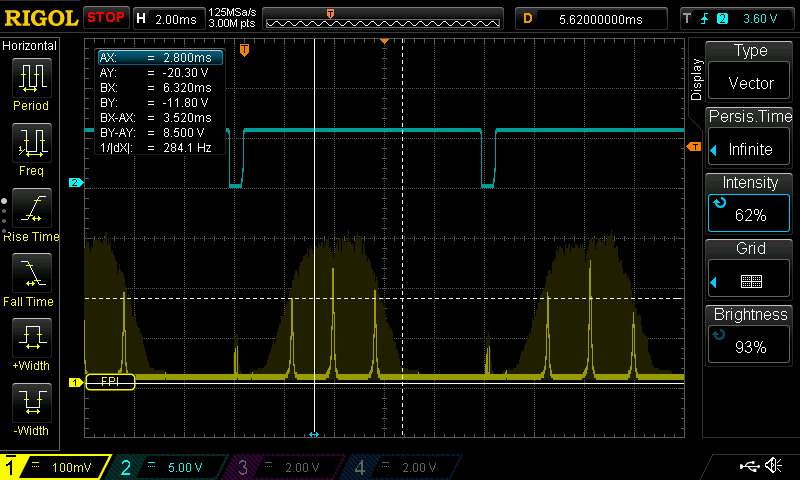
\includegraphics[width = \linewidth]{Bilder/Auswertung/FabryPerotVerst.png}
    \caption{Longitudinale Lasermoden mit dem Fabry-Pérot aufgenommen. Durch Erschütterung wurde das Verstärkungsprofil sichtbar gemacht.}
    \label{bild:Verstaerkung}
\end{figure}

Von diesem schätzen wir die Halbwertsbreite ab, soweit das geht. Die Halbwertsbreite 

\begin{equation}
    \textcolor{red}{\Delta \nu_{Verstärkungsprofil} = 532\pm80\;\mathrm{MHz}}
\end{equation}

hat einen relativ großen Fehler, da man die Spitze des Verstärkungsprofils nicht genau sehen kann und daher abschätzen muss.
Dies ist auch sinnvoll, da die Breite des Verstärkungsprofils mehrmals den Modenabstand beinhalten sollte.


\subsection*{Finesse und Auflösungsvermögen}

Die Finesse und das Auflösungsvermögen sind zwei Größen, die zur Charakterisierung des Resonators nützlich sind. Die Finesse ist dabei
definiert über das Verhältnis 
\begin{align}
    \mathcal{F} = \frac{\delta \nu_{FSR}}{\Delta\nu} \qquad s_{\mathcal{F}} = \sqrt{(\frac{s_{\Delta \nu}*\delta \nu_{FSR}}{\Delta\nu^2})^2+(\frac{s_{\delta\nu}}{\Delta \nu})^2}
\end{align}
 des freien Spektralbereichs zur Linienbreite. Die Auflösung 

 \begin{align}
     A = \frac{\nu}{\Delta\nu} = \frac{c}{\lambda\Delta\nu} \qquad s_A = A\sqrt{()\frac{s_{\Delta\nu}}{\Delta\nu})^2} = A\frac{s_{\Delta\nu}}{\Delta\nu}
 \end{align}
 
 ist hingegen das Verhältnis der Linienbreite zur Frequenz der Spektrallinie. Dabei wurde die Frequenz in
 die Lichtgeschwindigkeit 
% Gaussstrahlen

\section{Gaußstrahlen}
\label{sec:gauss}


\section{Hologramm}

Ein Hologramm ist in gewissem Sinne die Weiterentwicklung des Photos. Während bei einem Schwarzweißfilm nur die Intensität 
des Wellenfeldes gemessen wird, misst ein Farbphoto schon die Wellenlänge des verwendeten Lichtes mit. Das Hologramm 
beinhaltet nun außerdem Informationen über die Phase des Lichtes. Damit lässt sich ein dreidimensionales Abbild des 
Objektes rekonstruieren. Dabei wird das Hologramm mit einer bestimmten Quelle, der Referenzquelle, aufgenommen. Will man diese nun wiedergeben, benötigt man 
die Referenzquelle oder eine gleichartige Quelle. Wir haben hier ein Hologramm untersucht. Dieses zeigt einen Schlumpf 
beim Fußballspielen, was man in Abbildung \ref{bild:Holo} bewundern kann. 

\begin{figure}[ht]
    \centering
    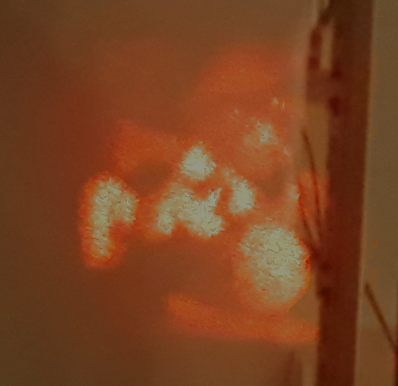
\includegraphics[width = 12cm]{Bilder/Auswertung/Holo.png}
    \caption{Hologramm mit einem HeNe-Hilfslaser aufgenommen}
    \label{bild:Holo}
\end{figure}

Dabei ist das Hologramm leider nicht optimal zu sehen, da wir nur den Hilfslaser verwenden konnten. Trotzdem sieht
man auch in Abbildung \ref{bild:Holo} die dreidimensionale Darstellung des Bildes.


% etc.

    % 5.Kapitel Fazit
    %Matteo Kumar - Leonard Schatt
% Fortgeschrittenes Physikalisches Praktikum

% 5. Kapitel Einleitung

\chapter{Fazit}
\label{chap:fazit}

Nach diesem Versuch können wir mit Sicherheit sagen, dass die Darstellung des Lasers in der Kunst eine Missrepresentation
des sehr beeindruckende Gerätes und Prozesses LASER ist. Ein Laser macht werder besonders futuristische Geräusche noch 
lässt er sich entspannt ohne Pumpe in ein Lichtschwerter einbauen. Dies hat uns der Versuch beigebracht. Des Weiteren hat
er uns einen verantwortungsvollen Umgang mit Lasern näher gebracht und seine Bedeutung in den Naturwissenschaften, insbesondere der Physik.

    % Charlotte Geiger - Manuel Lippert - Leonard Schatt
% Physikalisches Praktikum

% Anhang

\appendix

% Text

% Matteo Kumar - Leonhard Schatt
% Fortgeschrittenes Physikalisches Praktikum


% Anhang A

\chapter{Append A}
\label{chap:anhangA}

\section{Teilanhang X}


    % Literatur
    \bibliographystyle{Auswertung.bst}
    %\nocite{*}
    \bibliography{Auswertung.bib}

\end{document}